\documentclass[xcolor={dvipsnames},aspectratio=169,10pt]{beamer}
\usetheme{mx}
\usepackage{graphicx}
\graphicspath{{figures/}}
%\input{preamble.tex}

\title{
Teaching AI and Robotics to Children in a Mexican town
}
\subtitle{
Equity and Diversity in Design, Application, Methods, and Community \\
\#DEI-HRI2023 Workshop 
}

\author{
Antonio Badillo-P\'erez,
Donato Badillo-P\'erez, 
Alex Barco, \\ 
Rocio Montenegro, and
{\bf Miguel Xochicale}
}

\date{
%Workshop on Child-Robot Interaction \& Child's Fundamental Rights at 
%March 08, 2021
}

\institute{
	\faEnvelope \space  air4children@gmail.com \\
	\faGithubAlt \space @air4children \faTwitter \space @air4children  
		}

\titlegraphic{
  \begin{tikzpicture}[overlay, remember picture]
    \node[%
      above right=0.35cm and -0.2cm of current page footer area.south west,
      anchor=south west,
      inner sep=0pt] {%
      \usebeamerfont{footline}
      \begin{tabular}{lm{.8\textwidth}}
        \href{http://creativecommons.org/licenses/by/4.0/}{\ccby} &
        This slices is licensed under a
	\href{http://creativecommons.org/licenses/by/4.0/}
		{Creative Commons ``Attribution 4.0 International''} license. 
	\par Get source of this slides and see further references 
		from \url{https://github.com/air4children/dei-hri2023}.
      \end{tabular}
    };
    \node[%
      above left=0.35cm and 0cm of current page footer area.south east,
      anchor=south east,
      inner sep=0pt]{\qrcode[height=1.5cm]{https://github.com/air4children/dei-hri2023}};
  \end{tikzpicture}
}

\begin{document}

\maketitle

\begin{frame}{Table of Contents}
    \tableofcontents
\end{frame}

%%%%%%%%%%%%%%%%%%%%%%%%%%%%%%%%%%%%%%%%%%%%
\section{Background}


\begin{frame}
      \frametitle{Table of Contents}
      \tableofcontents[currentsection]
\end{frame}



%%%%%%%%%%%%%%%%%%%%%%%%%%%%%%%%%%%%%%%%%%%%%
\subsection{Education programs, publications and private investment in AI and Robotics}

%%%%%%%%%%%%%%%%%%%%%%%%%%%%%%%%%%%%%%%%%%%%%%%%%%%%%%%%
{
%\paper{Savage N. 2021 in Nature, DOI: doi.org/10.1038/d41586-020-03409-8}
\paper{Zhang D. et al 2021 in AI 2021 Index Report, Fig 4.3.3 https://aiindex.stanford.edu/report/}

\begin{frame}{Specialised AI programs by Geographic Area and level}

\begin{figure}
 \centering
 \includegraphics[width=1.0\textwidth]{./figures/progress-of-air-a/outputs/drawing-v00.png}
 %\caption{}
\end{figure}

\end{frame}
}


%%%%%%%%%%%%%%%%%%%%%%%%%%%%%%%%%%%%%%%%%%%%%%%%%%%%%%%%
{
%\paper{Savage N. 2021 in Nature, DOI: doi.org/10.1038/d41586-020-03409-8}
\paper{Zhang D. et al 2021 in AI 2021 Index Report, Fig 1.1.19 https://aiindex.stanford.edu/report/}

\begin{frame}{AI-related publications in arxiv by field of study}

\begin{figure}
 \centering
 \includegraphics[width=1.0\textwidth]{./figures/progress-of-air-b/outputs/drawing-v00.png}
 %\caption{}
\end{figure}

\end{frame}
}



%%%%%%%%%%%%%%%%%%%%%%%%%%%%%%%%%%%%%%%%%%%%%%%%%%%%%%%%
{
%\paper{Savage N. 2021 in Nature, DOI: doi.org/10.1038/d41586-020-03409-8}
\paper{Zhang D. et al 2021 in AI 2021 Index Report, Fig 1.1.19 https://aiindex.stanford.edu/report/}

\begin{frame}{Private investment in AI by Geographic area}

\begin{figure}
 \centering
 \includegraphics[width=1.0\textwidth]{./figures/progress-of-air-c/outputs/drawing-v00.png}
 %\caption{}
\end{figure}

\end{frame}
}



%%%%%%%%%%%%%%%%%%%%%%%%%%%%%%%%%%%%%%%%%%%%%
\subsection{Open source software and hardware in AI and Robotics}

%%%%%%%%%%%%%%%%%%%%%%%%%%%%%%%%%%%%%%%%%%%%%%%%%%%%%%%%
{
%\paper{Savage N. 2021 in Nature}
\begin{frame}{Open source software and hardware in AI and Robotics}

      \begin{figure}
        \centering
        \includegraphics[width=1.0\textwidth]{./figures/timeline-osh/outputs/drawing-v00.png}
        %\caption{}
      \end{figure}
\end{frame}
}


%%%%%%%%%%%%%%%%%%%%%%%%%%%%%%%%%%%%%%%%%%%%
\section{air4children}


\begin{frame}
      \frametitle{Contenido}
      \tableofcontents[currentsection]
\end{frame}


%%%%%%%%%%%%%%%%%%%%%%%%%%%%%%%%%%%%%%%%%%%%%
\subsection{
%Open source software and hardware in AI and Robotics
Software y hardware de fuente libre en IA y Rob\'otica
}

%%%%%%%%%%%%%%%%%%%%%%%%%%%%%%%%%%%%%%%%%%%%%%%%%%%%%%%%
{
%\paper{Savage N. 2021 in Nature}
\begin{frame}{
%Open source software and hardware in AI and Robotics
Software y hardware de fuente libre en IA y Rob\'otica
}

      \begin{figure}
        \centering
        \includegraphics[width=1.0\textwidth]{./timeline-osh/outputs/drawing-v00.png}
        %\caption{}
      \end{figure}
\end{frame}
}

%%%%%%%%%%%%%%%%%%%%%%%%%%%%%%%%%%%%%%%%%%%%%%%%%%%%%%%%
{
%\paper{Lastname N. YEAR in journal of...}
\begin{frame}{
air4children, 
Inteligencia Artificial y Rob\'otica para ni\~n@s
}
 
  \begin{columns}
  \begin{column}{.7\linewidth}

  \begin{itemize}
    %\item create a more inclusive, affordable and fair participation of children in AI and Robotics,
    \item crear talleres inclusivos, econ\'omicos y justo de IA y Rob\'otica para ni\~n@s, 
    %\item create child-centred AI and Robotics curriculums based on Montessori Education, and
    \item crear programas de IA y Rob\'otica basados en educaci\'on Montessori, y
    %\item build Open source robots to be affordable and fun. 
    \item construir robots de fuente libre econ\'omicos y divertidos.
  \end{itemize}

    \end{column}


  \begin{column}{.4\linewidth}

      \begin{figure}
        \centering
        \includegraphics[width=0.95\textwidth]{./logo/outputs/drawing-v00.png}
      \end{figure}

    \end{column}
  \end{columns}

\end{frame}
}




%%%%%%%%%%%%%%%%%%%%%%%%%%%%%%%%%%%%%%%%%%%%%
\subsection{
%Prototyping and piloting Open Source Robots
Prototipos y estudios piloto con Robots de fuente libre
}

%%%%%%%%%%%%%%%%%%%%%%%%%%%%%%%%%%%%%%%%%%%%%%%%%%%%%%%%
{
\paper{Xochicale M. June 2014, Proposal of Libre Robotics. 
\faFilePdfO Libre Robotics: \url{https://github.com/air4children/documents/blob/main/latex-librerobotics/LibrERobotics.pdf};
\faYoutube Voice Controlled Low-Cost Robot: \url{https://www.youtube.com/watch?v=f2mCCzVIxe0}
\faYoutube Robot learning: \url{https://www.youtube.com/watch?v=BKWucKcgsP0};
\faYoutube little robot: \url{https://www.youtube.com/watch?v=DexhVz_B8U0}
}
\begin{frame}{
%Prototyping Open Source Robots (2013 -- 2017)
Prototipos con robots de fuente libre (2013 -- 2017)
}
      \begin{figure}
        \centering
        \includegraphics[width=1.0\textwidth]{./air4children-a/outputs/drawing-v00.png}
        %\caption{}
      \end{figure}
\end{frame}
}

%%%%%%%%%%%%%%%%%%%%%%%%%%%%%%%%%%%%%%%%%%%%%%%%%%%%%%%%
{
\paper{Xochicale M. 2015 in Mecate; 
\faYoutube ROBIT @MECATE 2015 \url{https://www.youtube.com/watch?v=VjVGnwD422g};
Parra C. et al. 2016, \url{https://www.ottodiy.com/}
}
\begin{frame}{
%Piloting robot prototypes (2015 -- 2019)
Piloteando prototipos de robots de fuente libre (2015-2019)
}
      \begin{figure}
        \centering
        \includegraphics[width=1.0\textwidth]{./air4children-b/outputs/drawing-v00.png}
        %\caption{}
      \end{figure}
\end{frame}
}

%%%%%%%%%%%%%%%%%%%%%%%%%%%%%%%%%%%%%%%%%%%%%
\subsection{
M\'etodo Montessori
}

%%%%%%%%%%%%%%%%%%%%%%%%%%%%%%%%%%%%%%%%%%%%%%%%%%%%%%%%
{
\paper{
Elkin, M., Sullivan, A. and Bers, M.U. (2014). Implementing a Robotics Curriculum in an Early Childhood Montessori Classroom. Journal of Information Technology Education: Innovations in Practice, 13(1), 153-169. Informing Science Institute. \url{https://www.learntechlib.org/p/174845}.
}
\begin{frame}{
%Montessori Education
Educaci\'on Montessori
} 
\vspace{3mm}
%\it{
%"The hand is the instrument of the mind."
"Las manos son el instrumento de la mente"
%} 
%\\
Dr. Maria Montessori (1970-1952).

\vspace{2mm}
    \begin{figure}
        \centering
        \includegraphics[width=1.0\textwidth]{./montessori/outputs/drawing-v00.png}
        %\caption{}
      \end{figure}

Participaci\'on en exploraciones creativas para desarrollar habilidades motoras en actividades colaborativas y en equipo. 
\end{frame}
}



%%%%%%%%%%%%%%%%%%%%%%%%%%%%%%%%%%%%%%%%%%%%%%%%%%%%%%%%
{
\paper{
Mohammad Tarik, M., M. Zena Tarik, M. Zahraa Tarek, and M. Farah Tareq. "A Hybrid Spiral Project Based Learning Model for Microprocessor Course Teaching." DOI: \url{http://doi.org/10.24017/kjar}; 
Harden R.M. (1999) What is a spiral curriculum?, Medical Teacher, 21:2, 141-143, DOI: \url{https://doi.org/10.1080/01421599979752}
}
\begin{frame}{
M\'etodo de aprendizaje espiral 
}

  \begin{figure}
        \centering
        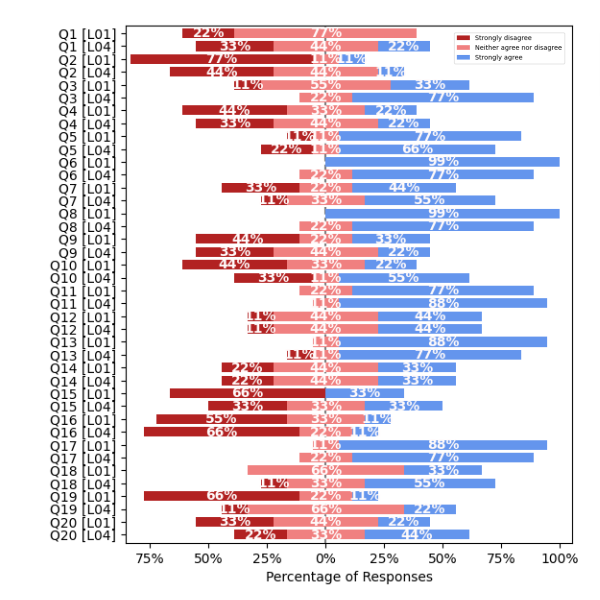
\includegraphics[width=1.0\textwidth]{./teaching-materials/outputs/drawing-v02.png}
        %\caption{}
      \end{figure}
\end{frame}
}

%%%%%%%%%%%%%%%%%%%%%%%%%%%%%%%%%%%%%%%%%%%%
\section{Workshops}


\begin{frame}
      \frametitle{Table of Contents}
      \tableofcontents[currentsection]
\end{frame}




%%%%%%%%%%%%%%%%%%%%%%%%%%%%%%%%%%%%%%%%%%%%%
\subsection{Four-lesson Curriculum}

%%%%%%%%%%%%%%%%%%%%%%%%%%%%%%%%%%%%%%%%%%%%%%%%%%%%%%%%
{
\paper{Badillo-Perez A, Badillo-Perez D, Barco A, Montenegro R, Xochicale M. 2013, Teaching AI and Robotics to Children in a Mexican town, DEI-HRI2023, \url{https://arxiv.org/abs/2303.03956}}

\begin{frame}{Curriculum}
      \begin{figure}
        \centering
        \includegraphics[width=1.0\textwidth]{./figures/curriculum/outputs/drawing-v00.png}
        %\caption{}
      \end{figure}
\end{frame}
}


%%%%%%%%%%%%%%%%%%%%%%%%%%%%%%%%%%%%%%%%%%%%%
\subsection{Piloting curriculum}

%%%%%%%%%%%%%%%%%%%%%%%%%%%%%%%%%%%%%%%%%%%%%%%%%%%%%%%%
{

\paper{Badillo-Perez A, Badillo-Perez D, Barco A, Montenegro R, \textbf{Xochicale M. 2023}, Teaching AI and Robotics to Children in a Mexican town, DEI-HRI2023, \url{https://arxiv.org/abs/2303.03956}}

\begin{frame}{Piloting workshop: Coding and bingo activities}
      \begin{figure}
        \centering
        \includegraphics[width=1.0\textwidth]{./figures/pilot-workshop-a/outputs/drawing-v00.png}
        %\caption{}
      \end{figure}
\end{frame}
}



%%%%%%%%%%%%%%%%%%%%%%%%%%%%%%%%%%%%%%%%%%%%%%%%%%%%%%%%
{

\paper{Badillo-Perez A, Badillo-Perez D, Barco A, Montenegro R, \textbf{Xochicale M. 2023}, Teaching AI and Robotics to Children in a Mexican town, DEI-HRI2023, \url{https://arxiv.org/abs/2303.03956}}

\begin{frame}{Piloting workshop: Teaching activities}
      \begin{figure}
        \centering
        \includegraphics[width=1.0\textwidth]{./figures/pilot-workshop-b/outputs/drawing-v00.png}
        %\caption{}
      \end{figure}
\end{frame}
}

%%%%%%%%%%%%%%%%%%%%%%%%%%%%%%%%%%%%%%%%%%%%%%%%%%%%%%%%
{

\paper{Badillo-Perez A, Badillo-Perez D, Barco A, Montenegro R, \textbf{Xochicale M. 2023}, Teaching AI and Robotics to Children in a Mexican town, DEI-HRI2023, \url{https://arxiv.org/abs/2303.03956}}

\begin{frame}{Piloting workshop: Group activities}
      \begin{figure}
        \centering
        \includegraphics[width=1.0\textwidth]{./figures/pilot-workshop-c/outputs/drawing-v00.png}
        %\caption{}
      \end{figure}
\end{frame}
}

%%%%%%%%%%%%%%%%%%%%%%%%%%%%%%%%%%%%%%%%%%%%%
\subsection{Results of the survey}

%%%%%%%%%%%%%%%%%%%%%%%%%%%%%%%%%%%%%%%%%%%%%%%%%%%%%%%%
{

\paper{Badillo-Perez A, Badillo-Perez D, Barco A, Montenegro R, \textbf{Xochicale M. 2023}, Teaching AI and Robotics to Children in a Mexican town, DEI-HRI2023, \url{https://arxiv.org/abs/2303.03956}}

\begin{frame}{Survey results}
      \begin{figure}
        \centering
        \includegraphics[width=1.0\textwidth]{./figures/survey-results/outputs/drawing-v00.png}
        %\caption{}
      \end{figure}
\end{frame}
}



%%%%%%%%%%%%%%%%%%%%%%%%%%%%%%%%%%%%%%%%%%%%
\section{Conclusions and Future work}


\begin{frame}
      \frametitle{Table of Contents}
      \tableofcontents[currentsection]
\end{frame}



%%%%%%%%%%%%%%%%%%%%%%%%%%%%%%%%%%%%%%%%%%%%%%%%%%%%%%%%
{
%\paper{Lastname N. YEAR in journal of...}
\begin{frame}{Conclusions and future work}

  \begin{columns}
  \begin{column}{.75\linewidth}

  \textbf{Conclusions}   

  \begin{itemize}
    \item Applied Montessory Education and spiral education to design child-based curriculumns in AI and Robotics
    \item Piloted a workshop with 14 participants of 4 lessons surveying attitudes with liker chart
  \end{itemize}

  \textbf{Future work}
  \begin{itemize}
    \item Improve surveys and statistical analysis
    \item Piloting AIR4Children with a major number of participants 
    \item Applying for funding 
    \item Engage with policy makers to increase the impact of air4children
\end{itemize}

    \end{column}


  \begin{column}{.3\linewidth}

      \begin{figure}
        \centering
        \includegraphics[width=0.9\textwidth]{logo/outputs/drawing-v00.png}
      \end{figure}

    \end{column}
  \end{columns}

\end{frame}
}


%%%%%%%%%%%%%%%%%%%%%%%%%%%%%%%%%%%%%%%%%%%%%%%%%%%%%%%%%
%{
%%\paper{Lastname N. YEAR in journal of...}
%\begin{frame}{Acknowledgements}
%
%  \begin{figure}
%  \centering
%  \includegraphics[width=1.0\textwidth]{./figures/team/outputs/drawing-v00.png}
%  \end{figure}
%
%\end{frame}
%}
%



%\begin{frame}
%  Thanks \\
%  Questions?
%\end{frame}

\maketitle

\end{document}
